\chapter{Fabrication}
\label{chapter:fabrication}

\section{Overview}

The fabrication procedure for soft pneumatic actuators can often be tedious and time-consuming to create a high volume of identical actuators \cite{hu_precurved_2022}. When designing the circular actuator's fabrication process, we were faced with casting a long, non-conventionally shaped actuator and wanted the fabrication process to be easily repeatable for high-volume production. 

Inspired by the fabrication process of Harvard's soft pneumatic actuator \cite{galloway_mechanically_2013, polygerinos_modeling_2015}, we cast a hollow silicone tube inside 3D-printed molds using a removable insert. We developed the fabrication process for circular actuators to maintain a uniform semi-circular cross-section and maximize the initial bending angle. This chapter includes how we cast silicone, fabricate the mold and insert, add strain-limiting materials, seal the ends, and interface with the pressurization equipment. 

\section{Procedure}

We use a single-material casting procedure with 3D-printed molds to create the circular actuators. A two-piece insert snaps into the mold to form the inner chamber and comes apart for easy removal (Fig.~\ref{figure:fab}A). The insert is constrained in the center of the mold so that the silicone walls have a constant thickness along the actuator to prevent off-axis motion (Fig.~\ref{figure:fab}B). We mix, degas, and pour a two-part silicone (Smooth-On, Inc) into the mold (Fig.~\ref{figure:fab}C). After casting, we leave the silicone to cure at room temperature. 

After the silicone cures, we remove the actuator from the mold and cut away excess material (Fig.~\ref{figure:fab}D). We add a strip of fiberglass fabric (4 oz S-glass, US Composites) to the flat side of the cross-section with Sil-Poxy (Smooth-On, USA) (Fig.~\ref{figure:fab}E). We paint a small amount of Dragon Skin 10 Fast (SmoothOn, USA) over the fiberglass to ensure a secure attachment to the actuator (Fig.~\ref{figure:fab}F). 

After removing the insert, we seal both ends with the same silicone used for the actuator body using a 3D-printed mold (Fig.~\ref{figure:fab}G). To connect to the pressurization equipment, we puncture one side of the actuator with a machined barb. The interface is coated with Sil-Poxy to ensure an airtight connection (Fig.~\ref{figure:fab}H).

\begin{figure}[ht!]
    \centering
     \includegraphics[width=4.5 in]{images4/fab.jpg}
    \caption{The simple fabrication process of the circular actuator.}
    \label{figure:fab}
\end{figure}

\clearpage
\section{Casting Silicone}

The silicones chosen for this project were a platinum cure, two-part silicones from Smooth-On, Inc. We used five different silicones with Shore A Hardness ranging from 20--50: DragonSkin 20~(DS20), DragonSkin 30~(DS30), SmoothSil 940~(SS40), SmoothSil 945~(SS45), and SmoothSil 950~(SS50). The shore hardness of the actuator is related to the bending resistance: the stiffer the material, the more stress is required to achieve a particular strain. It is essential that any materials used during the mixing process are compatible with the silicones and will not impact the curing process. For example, materials with high sulfur content inhibit the curing process. We used popsicle sticks, metal spatulas, and plastic cups to mix uncured silicone. Fig. \ref{fig:castingstation} contains an image of the casting station. 

\begin{figure}[ht]
    \centering
    \includegraphics[width=4 in]{images4/castingstation.jpeg}
    \caption{Photo of the casting station featuring DS20 silicone.}
    \label{fig:castingstation}
\end{figure}

Once we thoroughly mixed the two silicone parts, we degassed the mixture in a vacuum chamber for 2-3 minutes or until all the large air bubbles evacuated the mold. It is important to remove any air from the silicone. If the silicone cures around the air bubbles, the voids will disrupt the uniform cross-section required for consistent bending behavior. 

For each actuator, we used 40~g of part A and 40~g of part B of DS20 or DS30  silicone to fill the mold. To hold the molds together, we used several clamps to minimize the flashing and ensure a uniform cross-section. We poured the silicone a small amount at a time, ensuring all air bubbles could rise to the top. When pouring silicone, if the silicone ribbon gets too thin, more air is introduced as it folds onto itself. Frequent tapping of the mold on the lab bench was required to ensure that all of the air escaped. 

\section{Mold Design}

The mold design requirements include a pour hole large enough for us to cast silicone, a location for the insert to lock in, a path for all air to escape during casting, and useability for a high volume of actuators. Fig. \ref{fig:firstmold} contains the first mold designed for casting the circular actuator, highlighting the large pour hole at the top, the path for air to escape, the slot for the insert to lock into, and the asymmetries at the bottom of the molds so that they fit together and so no silicone could leak from the bottom. 

The arch shape allows us to pour in silicone from the top, and with the help of gravity, the silicone flows down to each end of the actuator. The insert sits in the center of the mold to create an even semi-circular cross-section. Even though excess silicone would cure at the top of the mold, we could easily cut it away from the flat side of the actuator. 

\begin{figure}[!ht]
    \centering
    \includegraphics[width=5.5 in]{images4/firstmolddesign.jpg}
    \caption{Design for the first mold. A. Isometric view of the mold and insert. B. Front view of one side of the mold.}
    \label{fig:firstmold}
\end{figure}

\section{Mold Fabrication and Iteration}

We chose to 3D-print the molds with PLA (polylactic acid) filament. Both molds could fit on one 3D-printer bed (Fig. \ref{fig:newmolds}A), which saves time and resources when fabricating molds. The PLA molds were robust enough to be clamped together using c-clamps. Unfortunately, the molds trapped air at the top (in the center of the actuator) during casting. To remove the air pockets, we cut away a small portion of the PLA (Fig. \ref{fig:newmolds}B) and eventually printed molds with an even larger pour hole. After dozens of actuators, the areas where we placed the clamps would begin to buckle, and the molds would warp out of shape. Abnormalities in the mold caused increased flashing (generating more waste) and an uneven cross-section (which would lead to uneven bending behavior). 

The next iteration of the 3D-printed molds, pictured in Fig. \ref{fig:newmolds}C, also included markings for clamp placement. We placed the clamps in locations where the two halves of the mold touch so that no mold deformation would impact the actuator's wall thickness. Extra clamps on the interior section were required for the thinner silicones to reduce leakage and flashing (Fig. \ref{fig:newmolds}D). 

\begin{figure}[ht]
    \centering
    \includegraphics[width=6.5 in]{images4/newmolds.jpg}
    \caption{Mold Iteration. A. First 3D-printed molds B. Cut portion of pour hole to allow air to escape. C. Drawing of the newer molds with markings for clamp placement and a larger pour hole. D. Photo of additional clamps required on the interior.}
    \label{fig:newmolds}
\end{figure}

\section{Insert Design}

Similar to the molds, there are several requirements for the insert design. The insert has a semi-circular cross-section so that the hollow actuator has the desired semi-circular walls. The insert must be able to sit in the mold in the center so that we can create actuators with even wall thickness. After casting, the insert must be removable from the silicone to create a hollow actuator. The insert should also be easy to fabricate to ensure a high-volume fabrication process for the circular actuator. The insert's bending radius and semi-circular cross-section did not change during design iterations. Instead, we created inserts out of several different materials while developing the final fabrication process. 

\subsection{Dissolvable Inserts}

We used a dissolvable, 3D-printable material to ensure we could remove the insert from the casted silicone and that the insert would have the desired dimensions. Commonly used as support material for PLA 3D prints, PVA (Polyvinyl Alcohol) is a material that is soluble in water. Fig. \ref{fig:pvainsert} contains photos of the PVA insert and actuators fabricated with this method. 

\begin{figure}[!ht]
    \centering
    \includegraphics[width=5.5 in]{images4/pvainsert.jpg}
    \caption{Fabrication of PVA inserts: A. PVA insert printed with PLA support material. B. DS20 actuators after removing from mold. C. DS20 and SS45 actuators after removing excess silicone. D. Hollow actuators post hot water bath.}
    \label{fig:pvainsert}
\end{figure}

After confirming that the silicone could cure around this material, we printed the first inserts out of PVA using an Ultimaker 3D printer. For the support material, we used PLA filament. Since PVA is rigid, only 5-10\% infill was required. The higher the infill on the insert, the more time-consuming it would be to dissolve it. We dissolved these single-use inserts using a hot water bath, leaving a hollow actuator with the desired semi-circular dimensions. Even though there were no problems removing the insert from the silicone post-cure, printing a new insert for every actuator used a lot of material and was time-consuming. We could use the PLA molds to cast dozens of actuators, but a single-use insert did not align with the goal of simple mass production.

\subsection{Flexible Inserts}

To create an insert that could be used multiple times and easily removed from the silicone after casting, we fabricated inserts by 3D-printing with TPU (thermoplastic polyurethane), a flexible filament. The stiffness of the TPU insert could be tuned based on the infill percentage. At first, the inserts were printed on the bed horizontally with no support material. In this orientation, the semi-circular cross-section's overhang created inconsistencies in the 3D-printed cross-section. We began printing the inserts with TPU as support material to ensure an even cross-section. Photographs of the TPU insert fabrication process are in Fig. \ref{fig:tpuprocess}. \\

\begin{figure}[!ht]
    \centering
    \includegraphics[width=6.5 in]{images4/tpuprocess.jpg}
    \caption{Fabrication using a TPU insert and pins. A. 3D printing with TPU. B. The pins placed in the insert.  C. Post silicone cure. D. Removing excess silicone from the ends and pour hole area. E. Removing the pins and insert. F. Silicone with solid insert. G. Post patching the holes from the pins. H. Completed hollow actuator body.}
    \label{fig:tpuprocess}
\end{figure}

The drawback of TPU inserts was that even though they could be used to cast multiple actuators, the inherent flexibility of TPU led the inserts to lose their circular shape over time. To continue using TPU and combat its flexibility, we used pins to hold the insert within the mold. Using three sets of pins evenly spaced along the length of the actuator (Fig. \ref{fig:tpuprocess}B), we could ensure the TPU insert would remain in the center of the mold during silicone casting. The pins created a new problem of needing to patch the holes left behind in the silicone. After casting the actuator with the TPU insert and pins, we would insert a different, solid TPU insert into the hollow silicone (Fig. \ref{fig:tpuprocess}F) to patch the holes with additional silicone and maintain the desired cross-section. Mixing and casting more silicone to patch the holes was not ideal because of the additional time required for the silicone to cure. 

\subsubsection{SS45 Silicone}

The TPU insert with pins method successfully created an airtight actuator for the soft DS20 silicone. To test if the fabrication procedure would work for stiffer silicones, we cast an actuator out of SS45 silicone. SS45 is much stiffer and has a much higher viscosity than DS20. Despite tapping the mold on the lab bench to remove the trapped air bubbles, after the silicone cured, large bubbles at the top of the mold remained, and after inspection, we found air pockets throughout the actuator. A more significant issue was that we could not remove the TPU insert. The silicone was too stiff for the end caps of the insert to slide through. We had to cut the silicone to remove the insert. Upon further inspection, a few air pockets remained inside of the silicone. Fig. \ref{fig:ss45mess} contains photos of testing the TPU insert and pins fabrication method for SS45 silicone. 

We also attempted to degas the mold after casting the SS45 actuator to combat the air holes that remained in the silicone. The small air pockets expanded, leaving the actuator with a significant amount of voids within the cross-section. Additionally, the pins left large holes, and since the solid TPU insert could not be slid in to patch the holes, we had to look into alternate methods of restricting the flexible insert. 

\begin{figure}[!ht]
    \centering
    \includegraphics[width=5.5 in]{images4/ss45mess.jpg}
    \caption{Images of failed SS45 actuator casting attempts. A. Overflow of mold during degassing. B. Samples of gaps created by air bubbles stuck in the mold. C. Un-patchable hole left from pin. D. Holes present in the actuator from over degassing}
    \label{fig:ss45mess}
\end{figure}

\subsubsection{Alternate Spacers with DS20}

For DS20 silicone, patching the holes left behind by the pins created an airtight seal. To remove the need to patch the holes, we attempted casting actuators using rings of DS20 silicone to hold the TPU insert in place. We printed a mold to cast small semi-circular rings of DS20 silicone, then cut a piece away so that the silicone would flow past the spacers and reach the ends while casting the actuator's body. The placement of the spacers was somewhat arbitrary as we were still determining if this method would create an airtight seal. After casting the actuator and removing it from the molds, simply pulling on it would break the seal between the silicone pieces cast at different times. Fig. \ref{fig:ds20spacer} contains images of this attempt centering the TPU insert inside the mold. 

\begin{figure}[ht!]
    \centering
    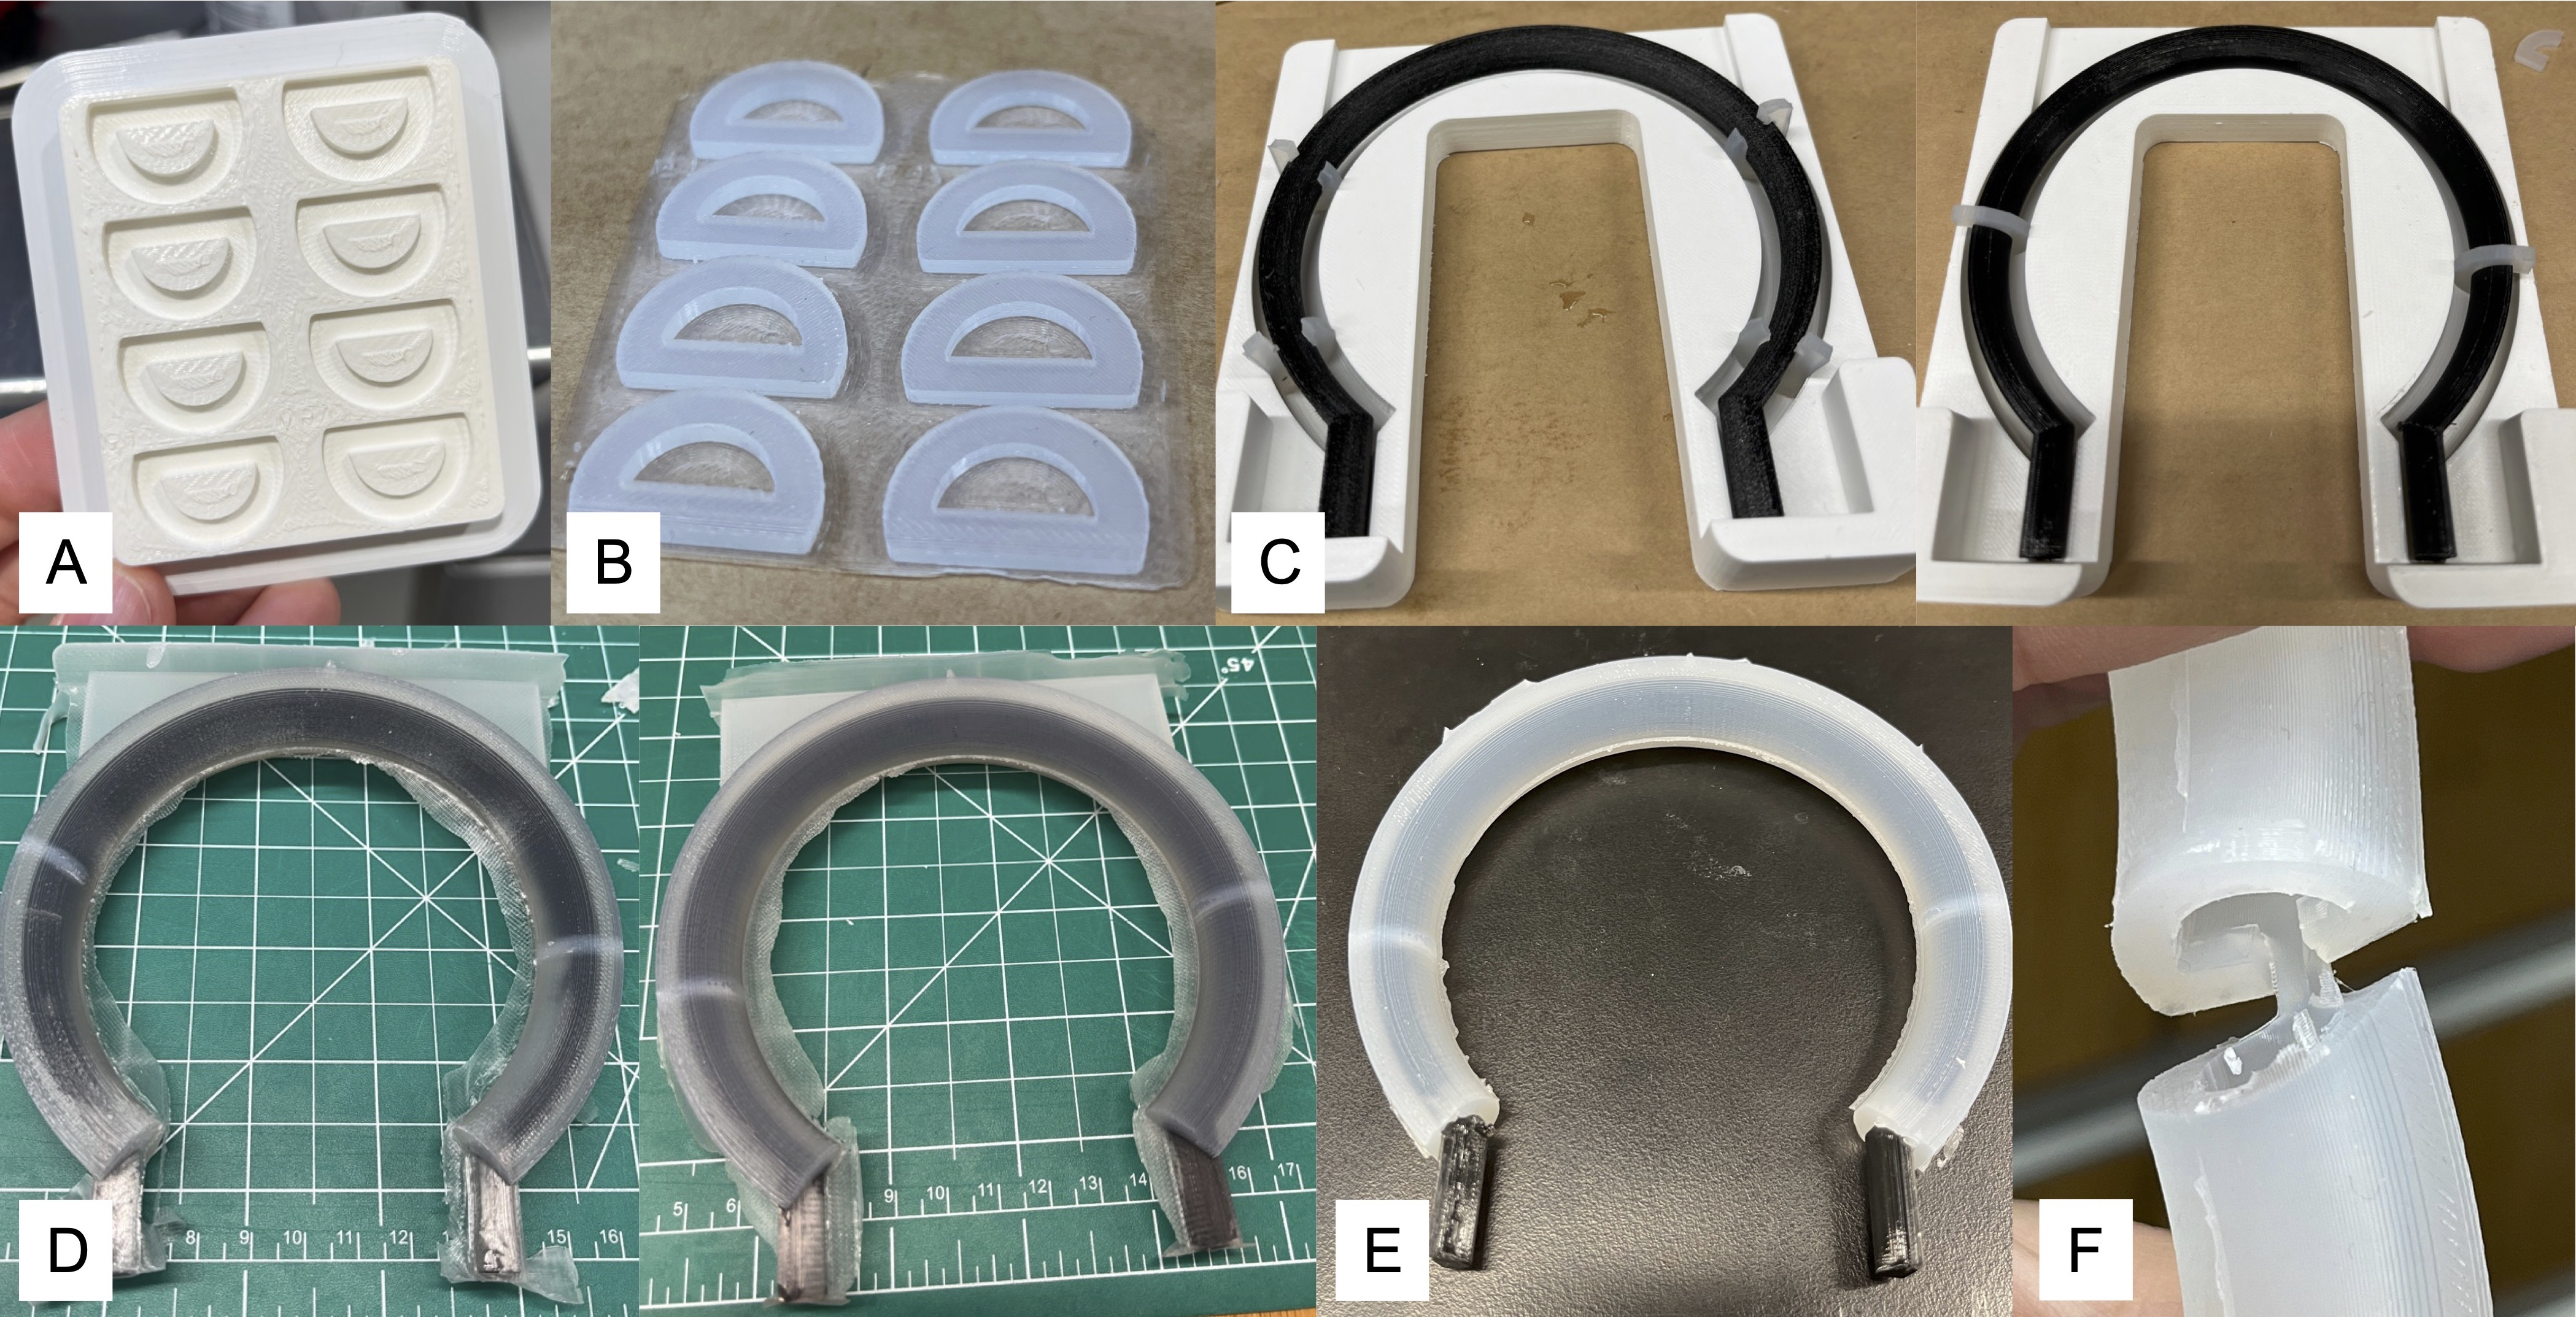
\includegraphics[width=5.5 in]{images4/ds20spacer.jpg}
    \caption{Images of failed attempts at using a spacer made from DS20 silicone to center the TPU insert. A. 3D printed mold for the spacers. B. Casted spacers. C. Arbitrary placement of spacers. D. Casted actuators right after removing from the mold. E. After removing excess silicone. F. Failed attempt at creating a seal.}
    \label{fig:ds20spacer}
\end{figure}

Overall, iterating with a flexible insert reaffirmed the need to cast the actuator's body in as few pours of silicone as possible to ensure the actuator would be airtight. Additionally, just because the insert works for the soft DS20 silicone does not necessarily guarantee that the insert will work for stiffer silicones. 

\clearpage
\subsection{Wax Inserts}

We fabricated wax inserts to create an insert that is more rigid than TPU but not as wasteful as PVA. We found three waxes compatible with curing silicone: beeswax, paraffin wax, and microcrystalline wax. We decided to cast the wax in a silicone mold for easy removal. To cast the silicone used as a mold, we 3D-printed a mold and insert out of PLA. Fig. \ref{fig:waxinserts} contains images from experimenting with wax inserts. 

\begin{figure}[ht!]
    \centering
    \includegraphics[width=5.5 in]{images4/waxinserts.jpg}
    \caption{Experimentation with wax inserts. A. 3D printed mold and insert for casting silicone mold for wax. B. Casting silicone mold. C. Paraffin wax casting. D. Paraffin insert removed from mold. E. Beeswax and microcrystalline wax casting. F. Beeswax and microcrystalline wax inserts.}
    \label{fig:waxinserts}
\end{figure}

All three waxes could be partially cast and removed from the silicone mold. However, we found that creating the wax insert to have the perfect cross-section shape to ensure a future uniform cross-section for the actuator was difficult, and the waxes were not rigid enough to hold their shape inside the DS20 mold during casting. We considered combining waxes in different ratios to enhance the stiffness and ease of casting. We also attempted fabricating inserts from polycaprolactone (PCL), (Appendix \ref{appendix:pcl}), but similar to wax inserts, even if they could create the perfect cross-section when casting silicone, they must be melted and recast to fabricate each actuator. 
With mass production in mind, we decided not to pursue wax or PCL inserts. 

\subsection{Two-Part PLA Inserts}

Reexamining the requirements for the insert design, we want an insert we could use for multiple actuators, and that creates a constant cross-section along the actuator. For the TPU insert, the ends with a different geometry than the cross-section of the actuator could not slide through stiffer silicones. If we split the insert along the section with the semi-circular cross-section, we could remove each part of the insert separately, and the silicone would not have to stretch during this process. 

To align the parts of the insert with each other, we added a connection point in the middle of the insert. Because the casted silicone picks up the filament lines, and 3D-printing the inserts with the large overhang without support material would cause inconsistencies in the cross-section, we attempted printing inserts in several orientations. Fig. \ref{fig:splitinsert} contains photographs of the possible orientations for 3D printing the split insert and actuators fabricated with this method. After 3D printing, we would also file and sand the inserts to ensure a smooth surface for the silicone to cast around. Fig. \ref{fig:splitinsert}A and B's 3D-printing orientation was difficult to smooth because the orientation of the layers meant more lines of filament on the sides of the insert, which made the silicone uneven on the inner wall. Fig. \ref{fig:splitinsert}C's orientation, the same method used for printing the PVA and TPU inserts, was the best because the lines of filament were aligned with the length of the actuator, creating a smoother inner surface. We use Teflon tape, which has a small width and smooth surface, to seal the interface between the two halves of the insert. \\

\begin{figure}[ht!]
    \centering
    \includegraphics[width=6.5 in]{images4/splitinsert.jpg}
    \caption{Photographs of the 2 part insert method. A-C. Three orientations for 3D printing the insert. D-G. DS20, DS30, SS40, and SS50, respectively, cast using inserts printed in the orientation shown in C.}
    \label{fig:splitinsert}
\end{figure}

Unfortunately, the silicone was not curing all the way in the areas where the tape touched the silicone. Moving the split of the insert to the edge of the actuator, an area of silicone that we would cut away before sealing the ends, significantly improved the bending behavior by ensuring an even cross-section of silicone along the length of the actuator. 

\clearpage
\section{Adding Strain Limiting Materials}

Now that we could consistently create circular actuators with a uniform cross-section in a single pour, the next problem was attaching the fiberglass fabric to the flat side of the silicone, a requirement for achieving the desired bending behavior with actuation. We used a large fiberglass fabric sheet (4 oz S-glass, US Composites) and cut it into strips slightly wider than the actuator to cover the entire flat face in fibers. We used Sil-Poxy (Smooth-On) to adhere the fabric to the silicone. We left the rigid PLA inserts inside the actuator while attaching the fiberglass fabric to ensure we added no stress to the silicone. Additionally, the fibers were attached parallel to the actuator to ensure the strain would be limited axially. If the fibers in the fabric are not aligned with the axial deformation the fiberglass is designed to restrict, the actuator will bend and twist in different directions with pressurization. 

Unfortunately, the Sil-Poxy adhesive was not strong enough on its own to keep the fiberglass attached, so we had to develop a way of covering the fabric in silicone to ensure the fabric would not become loose against the exterior of the actuator. In the standard fiber-reinforced actuator, a thin silicone wall is cast around the fiberglass, encasing the entire actuator. 

We attempted to design wider arch-shaped molds to cast another layer of silicone around the fiberglass, but this method was unsuccessful. Ensuring the second silicone cast had no air bubbles and completely covered the actuator was challenging due to the desired wall thickness. Additionally, making the walls of the actuator thicker would require more air pressure to achieve the bending behavior. For the softer silicones, casting another layer would be possible, but for the thicker silicones, such as SS40 and SS50, pouring another layer would be next to impossible. We considered casting an outer layer of a different material around the actuator, such as a thin Ecoflex silicone. However, having the semi-circular cross-section made from two different materials adds unnecessary complexity. 

To keep the total fabrication time as fast as possible, we used DragonSkin 10 (DS10) Fast cure silicone to paint a thin layer over the fiberglass fabric. Fig. \ref{fig:fiberglass} contains photographs of actuators before adding the fiberglass and after coating the fabric with a thin layer of DS10 silicone. The cure time for the DS10 silicone is under 1 hour, and only a small amount is needed to encase the fiberglass. We placed the actuator with the coat of DS10 on the table to dry, which allowed gravity to make the wall of silicone thin, but left a small amount of DS10 on the side of the actuator resting on the table (Fig. \ref{fig:fiberglass}D). This method was simple to execute repeatably, allowing for a consistent connection between the fiberglass fabric and the silicone actuator. 

\begin{figure}[ht!]
    \centering
    \includegraphics[width=5.5 in]{images4/fiberglass.jpg}
    \caption{Process of adding strain limiting fiberglass: A. Cut away silicone from flat side. B. After adding fiberglass to an SS40 actuator. C. After adding fiberglass to DS20. D. DS20 actuator right after the DS10 cured. E. After removing excess DS10.}
    \label{fig:fiberglass}
\end{figure}

\clearpage
\section{Sealing the Ends}

The easiest method to seal the ends is to place each end of the actuator in a cup full of silicone. While this method is the simplest, the amount of silicone pulled up the hollow actuator due to capillary effects is difficult to control. The larger the amount of silicone that forms the end cap, the more the final actuator's length decreases, which reduces the initial bending angle of the circular actuator. Additionally, there is an extra step to cut away the excess silicone cured around the end, leaving an end that is not necessarily uniform with the rest of the actuator. 

To ensure only the necessary amount of material cures inside the end of the actuator to create the end cap and maintain the actuator's clean cross-section, we designed and 3D printed a mold that matches the curvature of the circular actuator. Using these molds allowed us to cap the ends of all of our actuators with the same thickness on each end, further ensuring uniformity between the actuators. Fig. \ref{fig:endcaps} contains photographs of sealing the ends of the actuators and a drawing of the custom end cap mold used for the circular actuator. 

\begin{figure}[ht!]
    \centering
    \includegraphics[width=6 in]{images4/endcaps.jpg}
    \caption{Methods for sealing the ends of the actuator. A. Using a cup. B. Drawing of the custom mold. C. Sealing one end using the custom mold.}
    \label{fig:endcaps}
\end{figure}

\clearpage
\section{Connection to Pressurization Equipment}

We used standard tubing and push-to-connect fittings with 10-32 male threads to connect the actuator to the pressurization equipment. Fig. \ref{fig:barb} contains photos of the vented screw method and our custom barbs for connecting the actuator to the pressurization equipment. The vented screw method \cite{polygerinos_modeling_2015} involves using two pieces of laser cut acrylic, a vented screw, and a 10-32 nut to tighten the acrylic pieces around the end cap of silicone (Fig. \ref{fig:barb}C). Installation requires puncturing the vented screw through the inside of the actuator (Fig. \ref{fig:barb}A-B). A 10-32 female standoff connects the vented screw to the push-to-connect fitting (Fig. \ref{fig:barb}D). 

This method was successful for softer silicones, such as DS20. However, for stiffer silicones, puncturing with the vented screw often created a large hole in the end cap (Fig. \ref{fig:barb}B), which we attempted to seal with silicone glue with varying success. Additionally, puncturing from the inside, which requires feeding the vented screw through the entire length of the actuator, would prove difficult if we ever wanted to make the actuator longer and possibly spiral-shaped. 

To simplify the connection to the push-to-connect fitting, we designed and machined several barbs (Fig. \ref{fig:barb}E) from brass with 10-32 female threads that directly connected to the push-to-connect fittings (Fig. \ref{fig:barb}F). There are multiple benefits to using the barb over the vented screw. Firstly, the barb provided a way to clamp the actuator during testing. Also, puncturing the actuator from the outside allowed us to simplify the fabrication process further because we could cast the silicone on both end caps at the same time. Additionally, we have more control over the location of the puncture hole because we can see the insertion point. 

After puncturing the barb into the actuator, we used Sil-Poxy adhesive both underneath and around the brass barb to ensure an airtight connection. Also, we used a small amount of Kevlar thread to tie the end cap around the spikes of the barb. Adding the thread proved to be the most effective way of ensuring an airtight connection. 

\begin{figure}[ht!]
    \centering
    \includegraphics[width=5 in]{images4/barb.jpg}
    \caption{Methods for connecting the actuator to pressurization equipment. A. Vented screw and inner piece of acrylic. B. Large puncture hole for the stiffer SS45 silicone. C. Airtight DS20 actuator. D. 10-32 female standoff and push-to-connect fitting. E. Barbs machined for the circular actuator. F. Direct connection to push-to-connect fitting. G. Airtight SS50 and DS30 actuators. }
    \label{fig:barb}
\end{figure}